%%% Local Variables:
%%% mode: LaTeX
%%% TeX-master: t
%%% End:

\documentclass{beamer}

\usepackage[utf8]{inputenc}
\usepackage{graphicx}
\usepackage{tikz}

\usetikzlibrary {arrows.meta}

\usetheme{Berkeley}

%\useoutertheme{shadow}
%\useinnertheme{rounded}

\definecolor{BSUblue}{RGB}{0, 51, 160} % (primary)
\definecolor{BSUorange}{RGB}{214,67, 9} % (secondary)

\setbeamercolor{palette primary}{bg=BSUblue,fg=white}
\setbeamercolor{palette secondary}{bg=BSUblue,fg=white}
\setbeamercolor{palette tertiary}{bg=BSUblue,fg=white}
\setbeamercolor{palette quaternary}{bg=BSUblue,fg=white}
\setbeamercolor{structure}{fg=BSUblue} % itemize, enumerate, etc
\setbeamercolor{section in toc}{fg=BSUblue} % TOC sections

% Override palette coloring with secondary
\setbeamercolor{subsection in head/foot}{bg=BSUorange,fg=white}


%------------------------------------------------------------
%Title page
\title[TBD] {COOL PAPER TITLE}

\author[]
{Shane K. Panter\inst{1} \and Nasir, Eisty\inst{2}}

\institute[BSU]
{
  \inst{1}%
  Clinical Assistant Professor\\
  Boise State University
  \and
  \inst{2}%
  Assistant Professor\\
  Boise State University
}

\date[ESEM 24]
{International Symposium on Empirical Software Engineering and Measurement, October 2024}

\logo{
\includegraphics[height=1cm]{images/bsu-logo.eps}}

%End of title page configuration block
%------------------------------------------------------------


\begin{document}

\frame{\titlepage}

\section{Introduction}
\begin{frame}
  \frametitle{Introduction}
  \begin{tikzpicture}
    \node [inner sep=0pt,,outer sep=0pt,clip,rounded corners=0.5cm] (boise) at (0,0){
      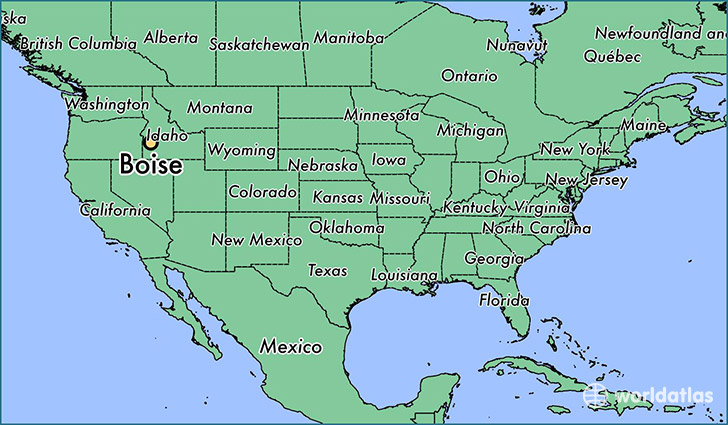
\includegraphics[width=0.8\textwidth]{images/boise-map.jpg}};

    \node [inner sep=0pt,,outer sep=0pt,clip,rounded corners=0.5cm] (ccp) at (3,-1){
      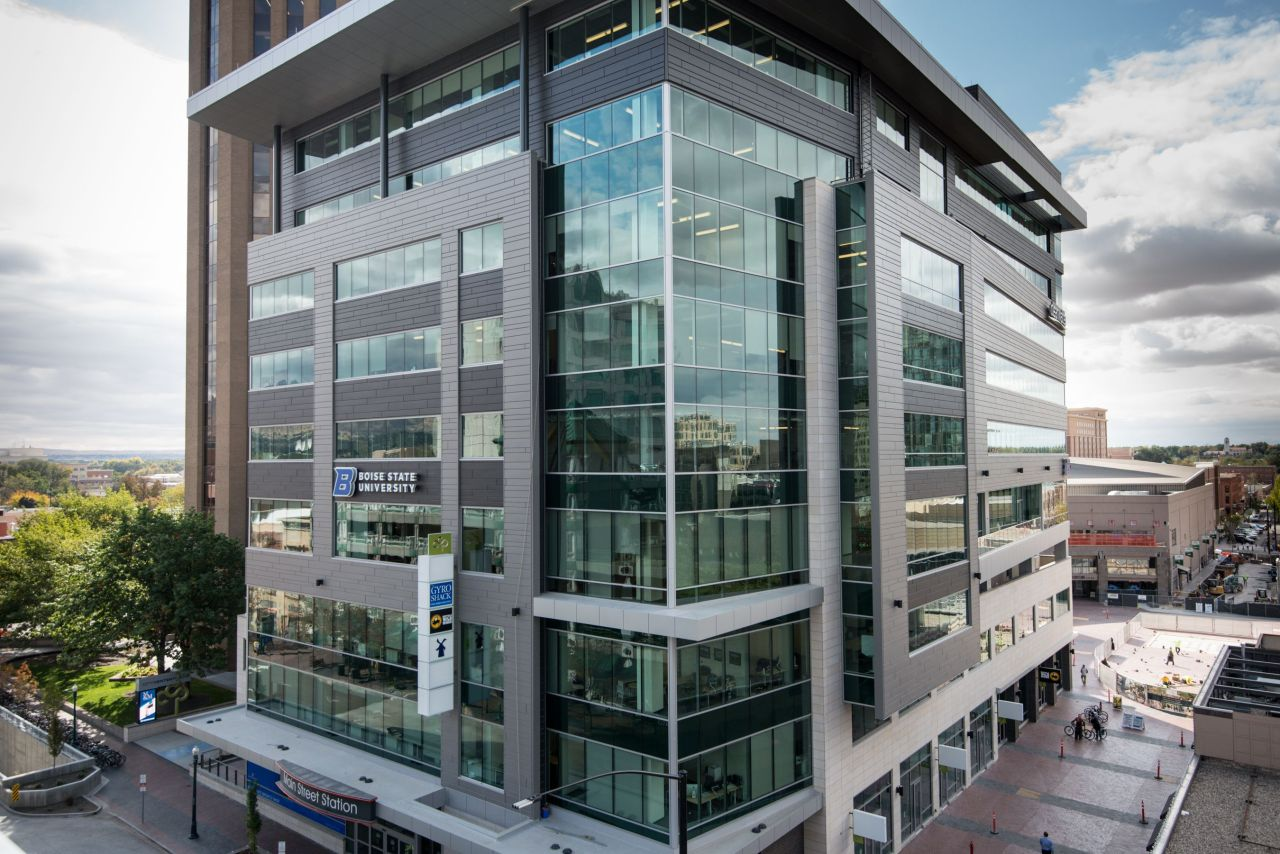
\includegraphics[width=0.45\textwidth]{images/CCP-from-northwest.jpg} };
    \draw[line width=4pt,
    arrows = {-Computer Modern Rightarrow[line cap=butt]}]       (ccp)   -- (-2.2,.8);

  \end{tikzpicture}

  \begin{block}{Boise State University}
    The Computer Science Department is located in Beautiful downtown Boise Idaho, United States!
  \end{block}

\end{frame}

\subsection{Our Research}


\begin{frame}
  \frametitle{Our Research}
  \begin{columns}
    \begin{column}{0.5\textwidth}

      TBD:

    \end{column}
    \begin{column}{0.5\textwidth}
      TBD:
    \end{column}
  \end{columns}

\end{frame}

\section{Methodology}

\subsection{Research Questions}
\begin{frame}
  \frametitle{Research Questions}
  \begin{itemize}
  \item<1-> \textbf{RQ1:} TBD
  \item<2-> \textbf{RQ2:} TBD
  \item<3-> \textbf{RQ3:} TBD
  \item<4-> \textbf{RQ4:} TBD

  \end{itemize}
\end{frame}

\subsection{Process Diagram}
\begin{frame}
  \frametitle{Process Diagram}
  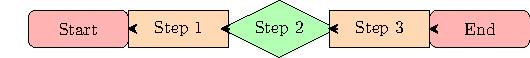
\includegraphics[width=4in]{figures/methodology.pdf}
\end{frame}
\section{Results}

\begin{frame}
  \frametitle{Results}
  \begin{columns}
    \begin{column}{0.5\textwidth}
      Our findings!
    \end{column}
    \begin{column}{0.5\textwidth}
      \begin{figure}
        \caption{Super happy researcher!\footnotemark[1]}
        
\includegraphics[width=.8\textwidth]{images/results.jpeg}\footnotemark[1]
      \end{figure}
    \end{column}
  \end{columns}
  \footnotetext[1]{AI Prompt: scientist getting research results and is super happy in a cyberpunk
    universe with lots of computers showing matrix code on them}
\end{frame}

\subsection{RQ1}
\begin{frame}
  \frametitle{RQ1}
\end{frame}

\subsection{RQ2}
\begin{frame}
  \frametitle{RQ2}
\end{frame}

\subsection{RQ3}
\begin{frame}
  \frametitle{RQ3}
\end{frame}

\subsection{RQ4}
\begin{frame}
  \frametitle{RQ4}
\end{frame}


\section{Conclusion}

\begin{frame}
  \frametitle{Conclusion}
\end{frame}

\section{Questions?}

\begin{frame}
  \frametitle{Questions?}
  \begin{columns}
    \begin{column}{0.5\textwidth}
      Questions?
    \end{column}
    \begin{column}{0.5\textwidth}
      \begin{figure}
        \caption{Happy People\footnotemark[1]}
        
\includegraphics[width=.8\textwidth]{images/questions.jpeg}\footnotemark[1]
      \end{figure}
    \end{column}
  \end{columns}
  \footnotetext[1]{AI Prompt: People attending a conference who all want to ask a question and are really excited!}
\end{frame}


\end{document}
